\section{Metodologia}

\subsection{Fenômeno de planagem}
    Neste experimento são utilizados dois modelos diferentes para simular o vôo de uma asa de avião. A versão mais simples consiste em um ventilados com as pás perpediculares a um aparato com uma face curva e outra reta. O aparato, doravante denominado ``asa'', tem fios atravessando verticalmente suas duas extremidades laterais ao longo do plano perpendicular às pás do ventilador. A asa fica orientada com a parte curva para cima e a parte reta para baixo. O modelo pode ser observado na \cref{asa_simples.png}.

    \begin{figure}[H]
        \centering
        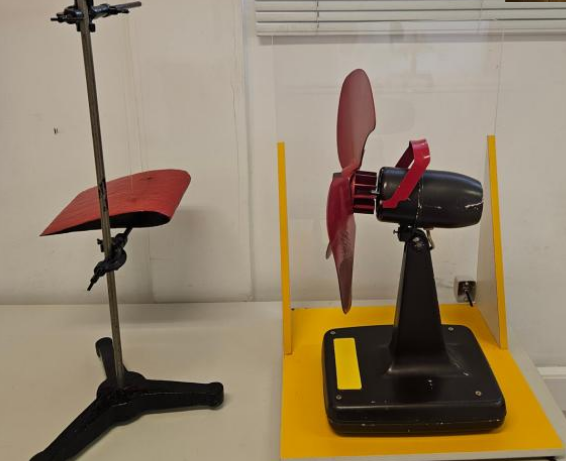
\includegraphics[width=0.35\linewidth]{fig/asa_simples.png}
        \caption{Modelo simples para estudo de planagem de uma asa de avião}
        \label{asa_simples.png}
    \end{figure}
    
    Já, a versão incluindo um tubo de pitot é construída também utilizando uma
    asa, porém com três furos, cada um conectado a um tubo. Os três
    tubos são paralelos ao plano das pás do ventilador, com sentido oposto ao
    vetor da aceleração da gravidade. Um dos furos tem saída para a parte mais
    próxima das pás do ventilador; outro para a parte curva da asa; e o terceiro
    para a parte reta da asa. É possível observar o perfil da asa e os furos na
    \cref{furos.png}. Assim como no modelo simplificado, a orientação da asa é
    tal que a parte curva fica para cima e a parte reta para baixo. Neste
    modelo, a asa fica dentro de um tubo de diâmetro igual ao diâmetro do
    ventilador posicionado à sua frente. Ademais, a asa fica presa por um
    mecanismo móvel externo ao tubo que contém o ventilador e a asa. Também, os
    tubos conectados aos furos na asa são finos e atravessam o tubo maior que
    contém o ventilador e a asa. À frente do tubo que contém o ventilador e a
    asa, coloca-se um manômetro líquido com um tubo flexível com comprimento
    suficiente para conectá-lo aos tubos dos furos da asa, um de cada vez. É
    possível observar o modelo com tubo de pitot na \cref{asa_pitot.png}.
    % Late night comment: Favor verificar o uso do termo paralelo quanto aos
    % tubos... -TF8 com sono

    \begin{figure}[H]
        \centering
        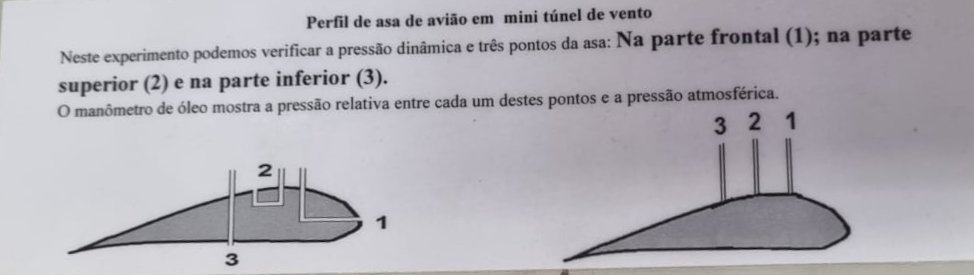
\includegraphics[width=0.35\linewidth]{fig/furos.jpeg}
        \caption{Perfil da asa de avião com tubo de pitot e descrição dos furos}
        \label{furos.png}
    \end{figure}
    \begin{figure}[H]
        \centering
        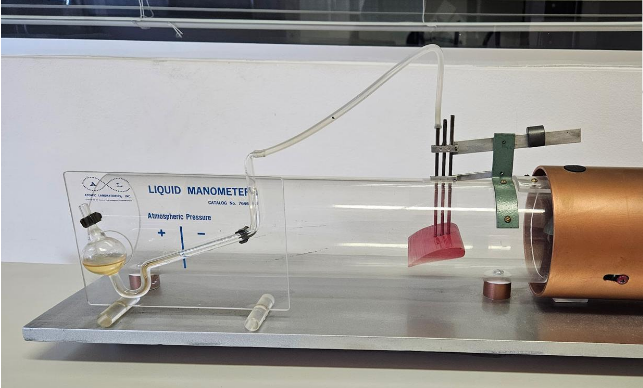
\includegraphics[width=0.35\linewidth]{fig/asa_pitot.png}
        \caption{Modelo com tubo de pitot para estudo de planagem de uma asa de avião}
        \label{asa_pitot.png}
    \end{figure}

    Para ambos os modelos, a observação é similar. No caso do modelo com tubo de pitot, primeiro deve-se conectar o tubo flexível do manômetro em um dos tubos conectados aos furos das asas. Em seguida, para ambos os modelos, deve-se ligar o ventilador e observar as variações resultantes. Em particular, para o modelo com tubo de pitot, é necessário repetir a experimentação com o manômetro conectado em cada um dos tubos.

\subsection{Tubos fechados com esferas}
    Para este experimento são utilizados dois tubos fechados, quase completamente preenchdios com líquido. Ambos os tubos têm marcações de distância a cada \(\qty{5}{cm}\). Além do líquido, em ambos os tubos, têm-se uma pequena esfera solta e uma bolha de ar, . Em um dos tubos há água, no outro um líquido indeterminado. Para a coleta de dados, uma câmera gravadora de vídeo é posicionada com a lente paralela a um dos tubos posicionado com o comprimento maior perpendicular ao plano do chão. Neste momento, a esfera deve estar na extremidade inferior. Então, inicia-se a gravação de vídeo e inverte-se o tubo. Posteriormente, é utilizado o software \textit{Tracker} para extrair informações de posição da esfera em relação ao tempo. O processo é repetido para o outro tubo. 

    %TODO: extrair uma imagem legal dos tubos dos vídeos e por aqui.
\subsection{Viscosímetro de Stokes}
    Neste experimento, utiliza-se um viscosímetro de Stokes, conforme observado na \cref{viscosimetro.png}, além de esferas de aço de diâmetro nominal variados e um funil. A temperatura do líquido é medida colocando um termômetro digital dentro do líquido pelo topo do tubo. Similarmente, a densidade é medida com um densímetro também inserido diretamente no líquido pelo topo do tubo. O diâmetro do tubo é medido utilizando um paquímetro. Ademais, o diâmetro das esferas é medido com um micrômetro. Para cada diâmetro nominal de esfera, são medidas e utilizadas quatro esferas. Ao montar o viscosímetro, é averiguado que esteja perpendicular ao plano do chão utilizando um prumo. 
    
    Para execução da experimentação, coloca-se o funil no topo do tubo do viscosímetro. Então, solta-se uma esfera imediatamente acima do funil. Deve ser cronometrado o tempo de queda da esfera de um ponto a outro, pré determinado e fixo para todas as esferar, do tubo do viscosímetro. O processo é repetido com cada esfera, anotando-se o tempo e o diâmetro nominal da esfera utilizada.  

    \begin{figure}[H]
        \centering
        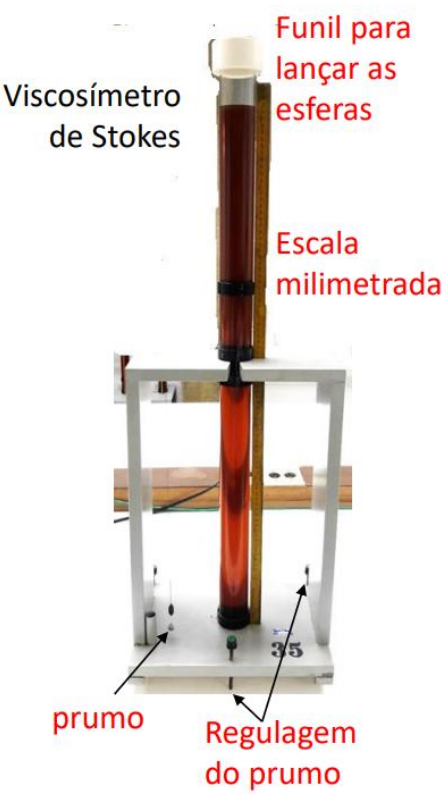
\includegraphics[width=0.3\linewidth]{fig/viscosimetro.png}
        \caption{Foto do viscosímetro de Stokes utilizado na experimentação incluindo descrição de todas as suas partes}
        \label{viscosimetro.png}
    \end{figure}

